
\subsubsection{Domain Class Diagrams}

The following class diagram provides a high-level view of the domain of interest for the \app platform. It is possible to notice elements that are external to the system (GitHub repositories, Users, Students, Educators) as well as the most meaningful internal ones (Tournaments, Battles, Scores, Rankings, Badges...). 
This diagram pursues the objective of showing the multiplicity relations between all of these components, along with the most relevant pieces of information (attributes) that characterize them.
As a remark to understand some of the multiplicity relations stated in the class diagram, only GitHub users that have already accessed \app once are considered, thus the 1:1 relationship between GitHubUser and User. Besides, the set of external GitHub repositories is restricted to those associated to a battle and the ones forked by the students from there.
\begin{center}
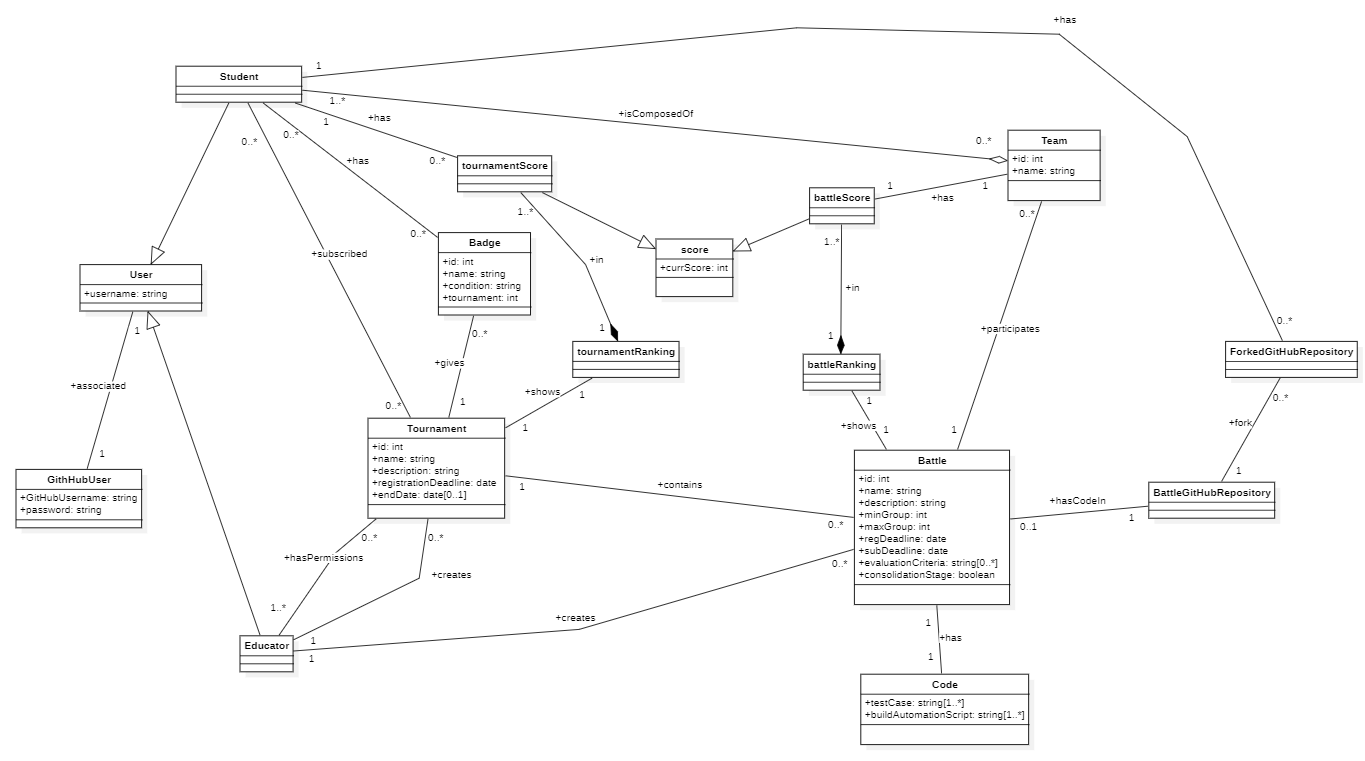
\includegraphics[angle=90,width=0.6\linewidth, scale=1.5]{2Overall_Description/res/ClassDiagram}
\end{center}


